% Paired contrasts transcribed from tex/main.tex, app:hidden-slice-exp.
% Endpoints are reported 95% Student-t CIs across five paired seeds.
\documentclass[tikz,border=0pt]{standalone}
% Shared publication style. Compile figure sources from this directory.
\usepackage[T1]{fontenc}
\usepackage{lmodern}
\usepackage{amsmath,amssymb}
\usepackage{tikz}
\usepackage{pgfplots}
\usetikzlibrary{arrows.meta,calc,positioning,backgrounds,patterns,shapes.geometric}
\usepgfplotslibrary{groupplots,fillbetween}
\pgfplotsset{compat=1.18}
\definecolor{fgblue}{HTML}{0072B2}
\definecolor{fgorange}{HTML}{D55E00}
\definecolor{fgslate}{HTML}{8B949E}
\definecolor{fgdark}{HTML}{25313C}
\definecolor{fgpale}{HTML}{F2F6F8}
\definecolor{fggrid}{HTML}{E3E8EC}
\definecolor{fgwater}{HTML}{D6EAF4}
\definecolor{fgland}{HTML}{E8E3D3}
\renewcommand{\familydefault}{\sfdefault}
\tikzset{every picture/.style={font=\fontsize{9}{11}\selectfont,text=fgdark},
  panel label/.style={font=\bfseries\fontsize{10}{12}\selectfont,anchor=north west},
  panel title/.style={font=\bfseries\fontsize{9}{11}\selectfont,anchor=north west},
  light arrow/.style={-{Stealth[length=1.6mm]},draw=fgslate,line width=.65pt}}
\pgfplotsset{fg axis/.style={
  axis line style={fgslate,line width=.4pt},axis x line*=bottom,axis y line*=left,
  tick align=outside,tick style={fgslate,line width=.4pt},
  tick label style={font=\fontsize{8}{10}\selectfont,text=fgdark},
  label style={font=\fontsize{9}{11}\selectfont,text=fgdark},
  title style={font=\bfseries\fontsize{9}{11}\selectfont,text=fgdark},
  grid style={fggrid,line width=.35pt},minor tick num=0,
  legend style={draw=none,fill=none,font=\fontsize{8}{10}\selectfont},
  scaled ticks=false,clip=false,
  every axis plot/.append style={line width=.85pt,mark size=2.2pt}
}}

\begin{document}
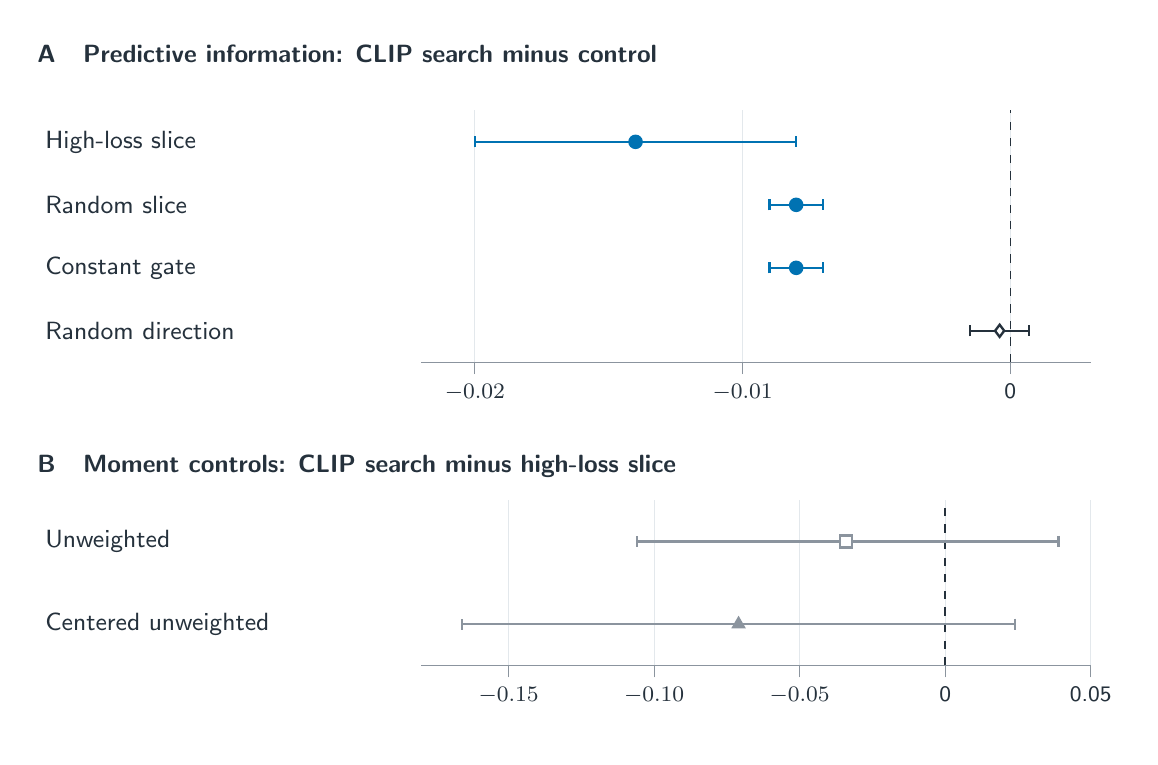
\begin{tikzpicture}[x=1mm,y=1mm]
\path[use as bounding box] (0,0) rectangle (140,90);
\node[panel title] at (0,89) {A\quad Predictive information: CLIP search minus control};
\node[anchor=west] at (1,75.5) {High-loss slice};
\node[anchor=west] at (1,67.5) {Random slice};
\node[anchor=west] at (1,59.5) {Constant gate};
\node[anchor=west] at (1,51.5) {Random direction};
\begin{axis}[fg axis,at={(50mm,47.5mm)},anchor=south west,
 width=85mm,height=32mm,scale only axis,
 xmin=-.022,xmax=.003,ymin=.5,ymax=4.5,axis y line=none,ytick=\empty,
 xtick={-.02,-.01,0},xticklabels={$-0.02$,$-0.01$,0},xmajorgrids=true,
 error bars/error bar style={line width=.85pt},
 error bars/error mark options={rotate=90,mark size=2pt,line width=.85pt}]
\draw[fgdark,dashed,line width=.5pt] (axis cs:0,.5)--(axis cs:0,4.5);
\addplot+[only marks,fgblue,mark=*,mark options={fill=fgblue},error bars/.cd,x dir=both,x explicit]
 coordinates {(-.014,4) += (.006,0) -= (.006,0)
 (-.008,3) += (.001,0) -= (.001,0)
 (-.008,2) += (.001,0) -= (.001,0)};
\addplot+[only marks,fgdark,mark=diamond*,mark options={fill=white},error bars/.cd,x dir=both,x explicit]
 coordinates {(-.0004,1) += (.0011,0) -= (.0011,0)};
\end{axis}
\node[panel title] at (0,37) {B\quad Moment controls: CLIP search minus high-loss slice};
\node[anchor=west] at (1,24.75) {Unweighted};
\node[anchor=west] at (1,14.25) {Centered unweighted};
\begin{axis}[fg axis,at={(50mm,9mm)},anchor=south west,
 width=85mm,height=21mm,scale only axis,
 xmin=-.18,xmax=.05,ymin=.5,ymax=2.5,axis y line=none,ytick=\empty,
 xtick={-.15,-.10,-.05,0,.05},xticklabels={$-0.15$,$-0.10$,$-0.05$,0,0.05},xmajorgrids=true,
 error bars/error bar style={line width=.85pt},
 error bars/error mark options={rotate=90,mark size=2pt,line width=.85pt}]
\draw[fgdark,dashed,line width=.5pt] (axis cs:0,.5)--(axis cs:0,2.5);
\addplot+[only marks,fgslate,mark=square*,mark options={fill=white},error bars/.cd,x dir=both,x explicit]
 coordinates {(-.034,2) += (.073,0) -= (.072,0)};
\addplot+[only marks,fgslate,mark=triangle*,mark options={fill=fgslate},error bars/.cd,x dir=both,x explicit]
 coordinates {(-.071,1) += (.095,0) -= (.095,0)};
\end{axis}
\end{tikzpicture}
\end{document}
